% Options for packages loaded elsewhere
\PassOptionsToPackage{unicode}{hyperref}
\PassOptionsToPackage{hyphens}{url}
\documentclass[
]{article}
\usepackage[a4paper, left=2.5cm, right=2.5cm, top=2.5cm, bottom=2.5cm]{geometry}
\usepackage{xcolor}
\usepackage{amsmath,amssymb}
\setcounter{secnumdepth}{-\maxdimen} % remove section numbering
\usepackage{iftex}
\ifPDFTeX
  \usepackage[T1]{fontenc}
  \usepackage[utf8]{inputenc}
  \usepackage{textcomp} % provide euro and other symbols
\else % if luatex or xetex
  \usepackage{unicode-math} % this also loads fontspec
  \defaultfontfeatures{Scale=MatchLowercase}
  \defaultfontfeatures[\rmfamily]{Ligatures=TeX,Scale=1}
\fi
\usepackage{lmodern}
\ifPDFTeX\else
  % xetex/luatex font selection
\fi
% Use upquote if available, for straight quotes in verbatim environments
\IfFileExists{upquote.sty}{\usepackage{upquote}}{}
\IfFileExists{microtype.sty}{% use microtype if available
  \usepackage[]{microtype}
  \UseMicrotypeSet[protrusion]{basicmath} % disable protrusion for tt fonts
}{}
\makeatletter
\@ifundefined{KOMAClassName}{% if non-KOMA class
  \IfFileExists{parskip.sty}{%
    \usepackage{parskip}
  }{% else
    \setlength{\parindent}{0pt}
    \setlength{\parskip}{6pt plus 2pt minus 1pt}}
}{% if KOMA class
  \KOMAoptions{parskip=half}}
\makeatother
\usepackage{longtable,booktabs,array}
\newcounter{none} % for unnumbered tables
\usepackage{calc} % for calculating minipage widths
% Correct order of tables after \paragraph or \subparagraph
\usepackage{etoolbox}
\makeatletter
\patchcmd\longtable{\par}{\if@noskipsec\mbox{}\fi\par}{}{}
\makeatother
% Allow footnotes in longtable head/foot
\IfFileExists{footnotehyper.sty}{\usepackage{footnotehyper}}{\usepackage{footnote}}
\makesavenoteenv{longtable}
\usepackage{graphicx}
\makeatletter
\newsavebox\pandoc@box
\newcommand*\pandocbounded[1]{% scales image to fit in text height/width
  \sbox\pandoc@box{#1}%
  \Gscale@div\@tempa{\textheight}{\dimexpr\ht\pandoc@box+\dp\pandoc@box\relax}%
  \Gscale@div\@tempb{\linewidth}{\wd\pandoc@box}%
  \ifdim\@tempb\p@<\@tempa\p@\let\@tempa\@tempb\fi% select the smaller of both
  \ifdim\@tempa\p@<\p@\scalebox{\@tempa}{\usebox\pandoc@box}%
  \else\usebox{\pandoc@box}%
  \fi%
}
% Set default figure placement to htbp
\def\fps@figure{htbp}
\makeatother
\setlength{\emergencystretch}{3em} % prevent overfull lines
\providecommand{\tightlist}{%
  \setlength{\itemsep}{0pt}\setlength{\parskip}{0pt}}
\usepackage{bookmark}
\IfFileExists{xurl.sty}{\usepackage{xurl}}{} % add URL line breaks if available
\urlstyle{same}
\hypersetup{
  hidelinks,
  pdfcreator={LaTeX via pandoc}}

\author{}
\date{}

\begin{document}

\begin{center}
    Universidad de Carabobo

Facultad de ciencias y tecnologia

Laboratorio nro.1 de Arquitectura del computador
\end{center}


estudiantes:

Jose Alvarez 31389258

Jose Nuñez 31581050

\begin{center}
Introducción
\end{center}


El presente laboratorio tiene como objetivo principal la inmersión en
los fundamentos de la programación en lenguaje ensamblador MIPS32,
utilizando el simulador MARS como entorno de desarrollo. La
implementación de algoritmos, tanto recursivos como iterativos, sirve
como vehículo para analizar la gestión de recursos a bajo nivel, un
aspecto crítico en la arquitectura de computadores.

A través de este ejercicio, se explora el comportamiendo del procesador
frente a la manipulación directa de registros y la gestión dinámica de
la memoria a través de la pila (\textbf{\$sp}). El análisis comparativo
entre ambos enfoques permitirá comprender las implicaciones de
rendimiento y seguridad que conlleva la elección de una estructura
algorítmica, estableciendo una base sólida para el desarrollo de
software eficiente en sistemas donde el control sobre el hardware es
absoluto.

1. ¿ Cómo se implementa la recursividad en MIPS32 ?

¿ Qué papel cumple la pila (\$sp) ?

R-

La recursividad en MIPS se implementa mediante la técnica de
auto-llamada, apoyada estrictamente en el estándar de llamadas
(\emph{Calling convention}).

- \textbf{Implementación}: Se define un \emph{Prologue} donde se
reservan espacios en la pila, se guarda la direccion de retorno
(\textbf{\$ra}) y los argumentos necesarios, y un \emph{Epilogue} donde
se restaura el estado previo antes de retornar (\textbf{jr \$ra}).

- \textbf{Papel de la pila} (\textbf{\$sp}): La pila actúa como una
``memoria temporal de historial''. En cada llamada recursiva,
\textbf{\$sp} se desplaza (decrementa en MIPS) para crear un nuevo marco
(\emph{stack frame}). Esto es vital porque el registro \textbf{\$ra}
solo puede almacenar una dirección a la vez; sin la pila, cada llamda
nueva sobreescribiría la dirección de retorno de la anterior, dejando al
programa ``perdido'' y sin forma de volver al flujo principal.

2. ¿ Qué riesgos de desbordamiento existen ?

¿ Cómo mitigarlos ?

R-

El riesgo principal es el \textbf{Stack Overflow} (desbordamiento de
pila).

- \textbf{El riesgo}: MIPS asigna un segmento de memoria finito para la
pila. Si la profundidad de la recursión es muy alta, el puntero
\textbf{\$sp} sigue restando direcciones hasta invadir segmentos de
memoria que no le corresponden (como los datos globales o el código).
Esto provoca una interrupción del programa (Runtime Exception).

- \textbf{Cómo mitigarlos}:

1- \textbf{Enfoque iterativo}: Siempre que sea posible, transformar el
algoritmo recursivo en uno iterativo para utilizar registros en lugar de
memoria de pila.

2- \textbf{Validacion de entrada}: Limitar el rango de entrada del
usuario para asegurar que nunca supere la capacidad de profundidad de la
pila.

3- \textbf{Tail Recursion} (\textbf{Recursión de cola}): Si el lenguaje
o el compilador lo permiten, optimizar la función para que la llamada
recursiva sea la última instrucción, permitiendo reutilizar el mismo
\emph{stack frame}.

3. ¿ Qué diferencias encontraste entre una implementación iterativa y
una recursiva en cuanto al uso de memoria y registros ?

{\def\LTcaptype{none} % do not increment counter
\begin{longtable}[]{@{}
  >{\raggedright\arraybackslash}p{(\linewidth - 4\tabcolsep) * \real{0.3333}}
  >{\raggedright\arraybackslash}p{(\linewidth - 4\tabcolsep) * \real{0.3333}}
  >{\raggedright\arraybackslash}p{(\linewidth - 4\tabcolsep) * \real{0.3333}}@{}}
\toprule\noalign{}
\endhead
\bottomrule\noalign{}
\endlastfoot
\textbf{Criterio} & \textbf{Implementación Recursiva} &
\textbf{Implementación Iterativa} \\
\textbf{Uso de memoria} & \emph{O(n)} (crece linealmente con \emph{n}) &
\emph{O(1)} (constante) \\
\textbf{Uso de registros} & Intenso(guardar/cargar en cada llamada) &
Mínimo (uso de registros temporales) \\
\textbf{Flujo de control} & Basado en llamadas (\textbf{jal}) & Basado
en saltos(\textbf{j}, \textbf{bnez}) \\
\end{longtable}
}

En la recursiva, el costo en memoria es alto debido al almacenamiento
constante de registros en la pila. En la iterativa, el estado del
programa se mantiene en registros internos (como \textbf{\$t0} o
\textbf{\$v0}), eliminando el costo de acceso a memoria ecterna.

4. ¿ Qué diferencias encontraste entre los ejemplos académicos del libro
y un ejercicio completo y operativo en MIPS32 ?

- \textbf{En la teoría}: Los libros a menudo ignoran la ``crudeza'' de
los regitros, asumiendo que el \emph{stack} es infinito o que el manejo
de registros es automático.

- \textbf{En la práctica}: En MIPS, el programador es responsable de
gestionar absolutamente todo: guardar registros que podrían ser
modificados por funciones llamadas, manejar manualmente el puntero de
pila y asegurar que \textbf{jal} tenga su correspondiente \textbf{jr
\$ra}. La diferencia es el nivel de control y, por ende, la
responsabilidad de evitar errores de segmentación.

5. Elaborar un tutorial de la ejecución paso a paso en MARS

Recursivo:

-Paso 1: Tras ensamblado el programa, este llega a la linea 10: y le
asigna a \$v0 el valor 4 (usado para escribir un string) para asi
escribir el texto ``Ingrese un numero entero positivo''.

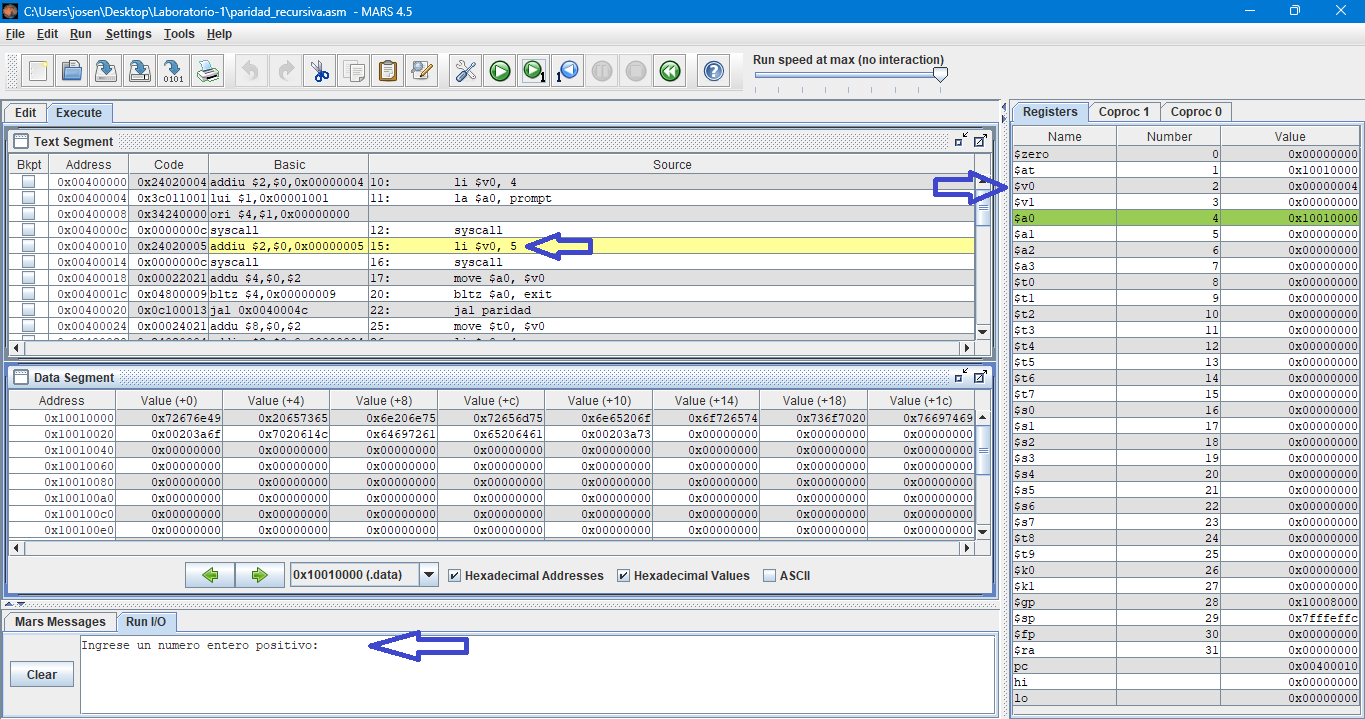
\includegraphics[width=1.0\textwidth]{./media/image1.png}

-Paso 2: Luego llega a la linea 15: y le asigna a \$v0 el valor 5 (usado
para recibir un entero) para asi esperar que el usuario ingrese un
numero.

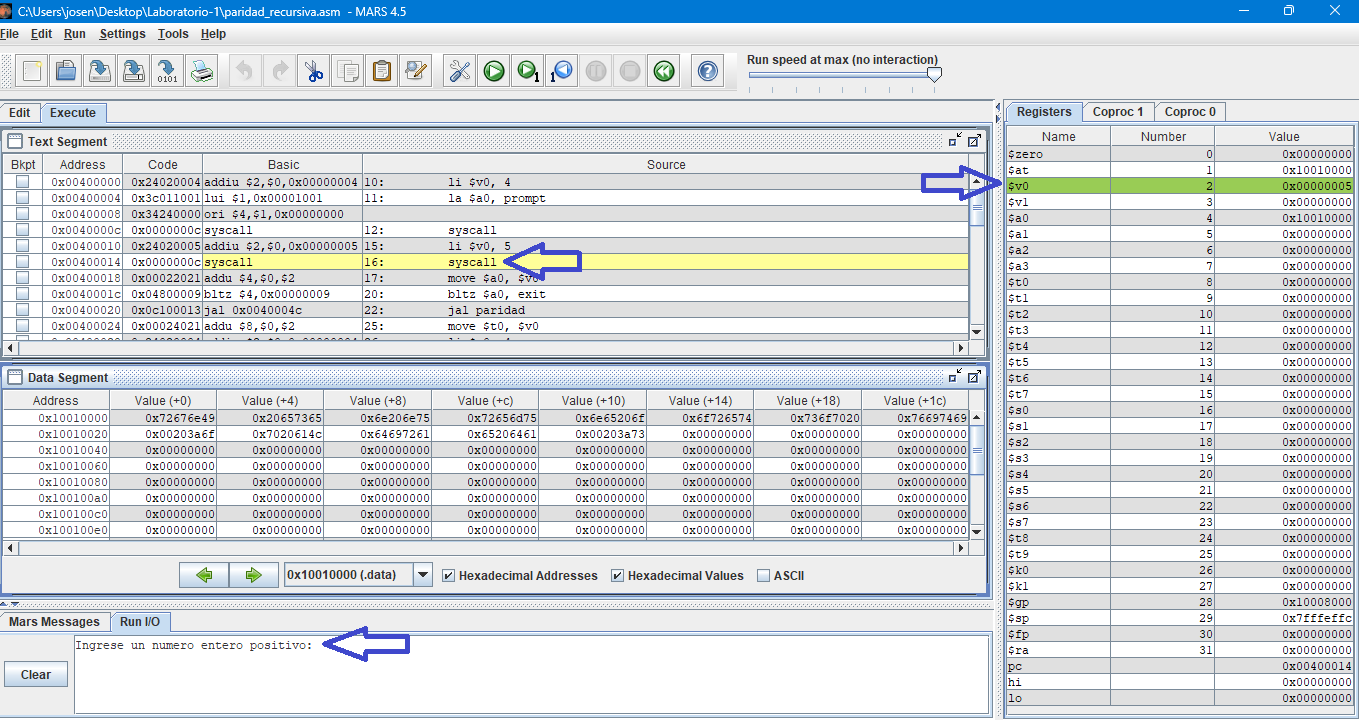
\includegraphics[width=1.0\textwidth]{./media/image2.png}

-Paso 3: Tras el usuario ingresar un valor (en este ejemplo ``2'') el
programa llega a la linea 17: y mueve el valor a la dirección del
registro \$a0.

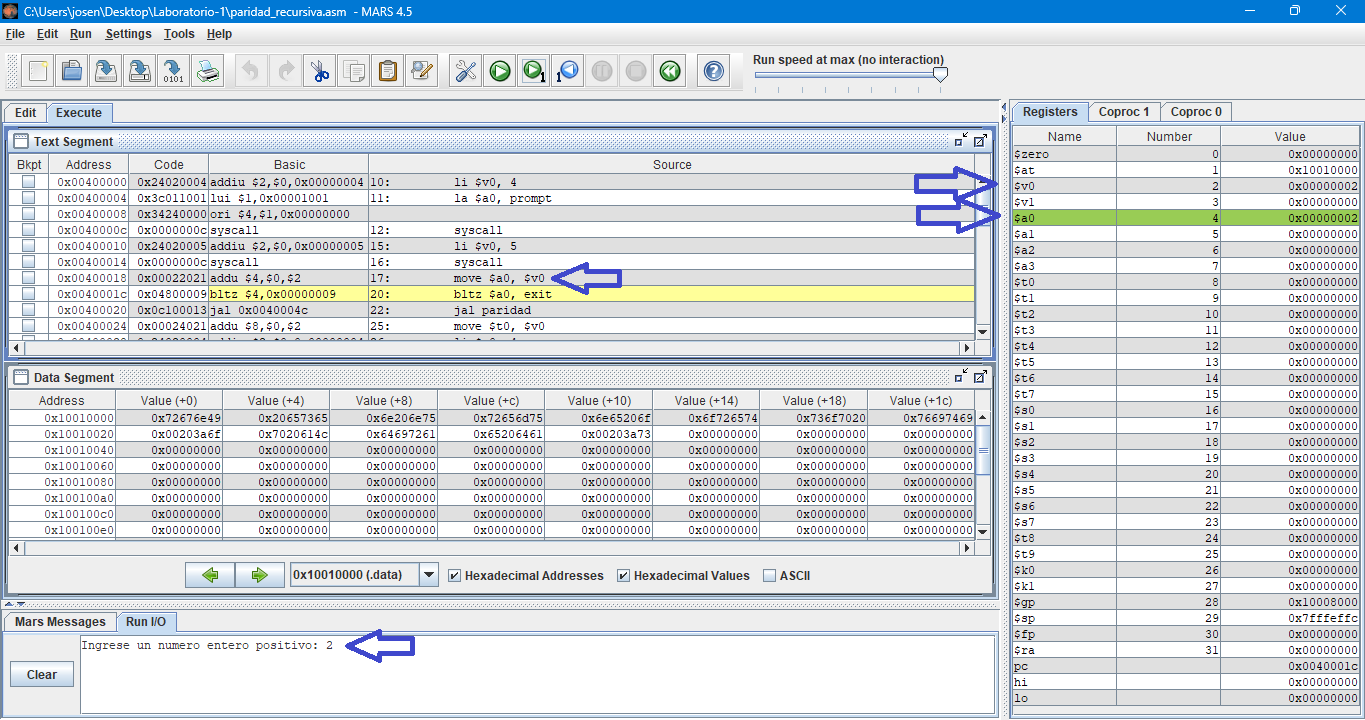
\includegraphics[width=1.0\textwidth]{./media/image3.png}

-Paso 4: El programa llega a la linea 22: y salta a la etiqueta
``\emph{paridad}'', en las lineas 41: a 43: guarda espacio en el puntero
\$sp para los registros \$a0 (el numero n) y \$ra (la memoria del paso
anterior para poder regresar).

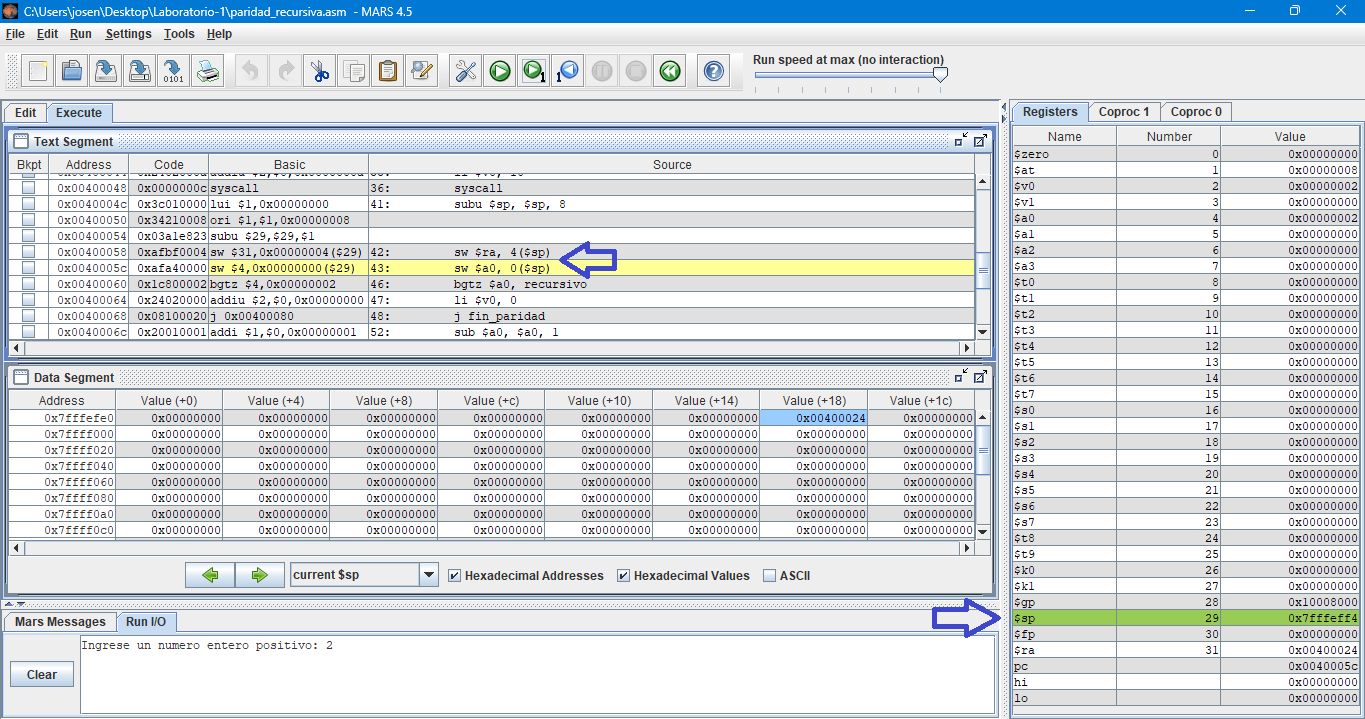
\includegraphics[width=1.0\textwidth]{./media/image4.png}

-Paso 5: El programa llega a la linea 46: y pregunta si \$a0 es mayor de
cero con la operacion bgtz. En este paso \$a0 es igual a dos por lo
tanto es verdad y salta hacia la etiqueta ``\emph{recursivo}''.

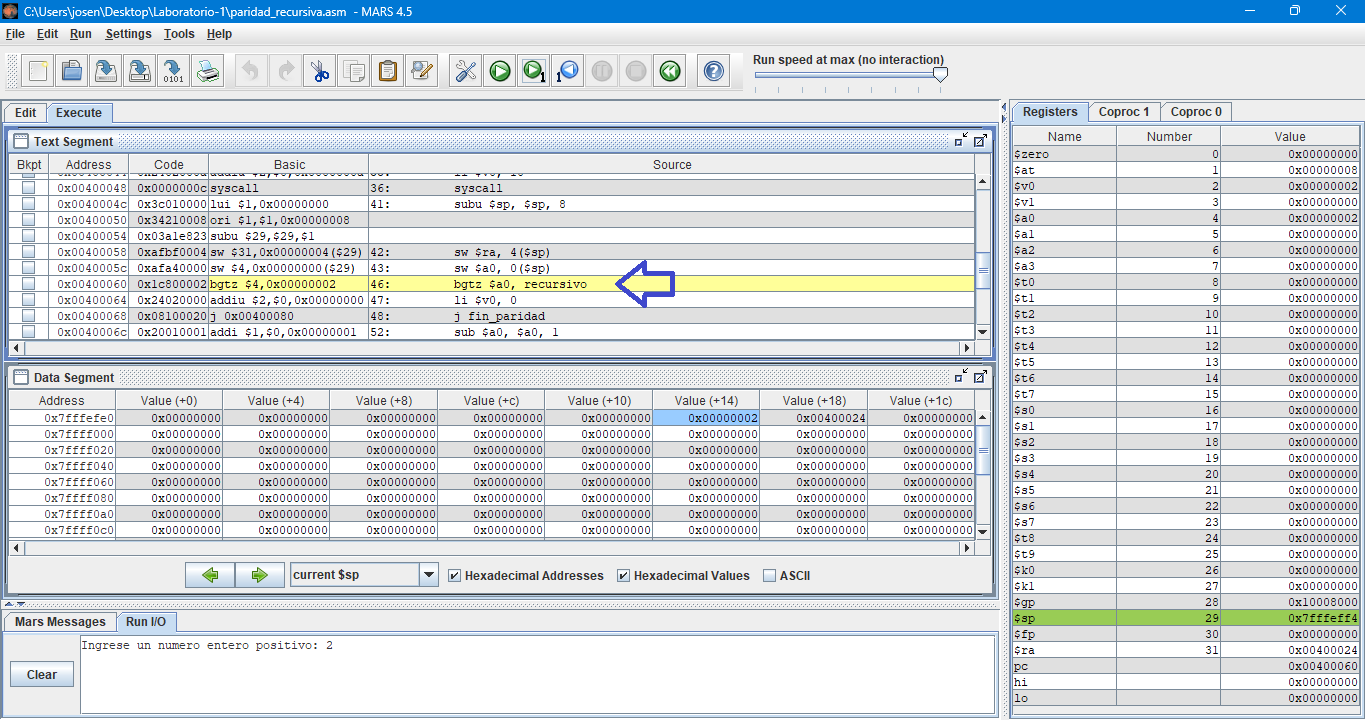
\includegraphics[width=1.0\textwidth]{./media/image5.png}

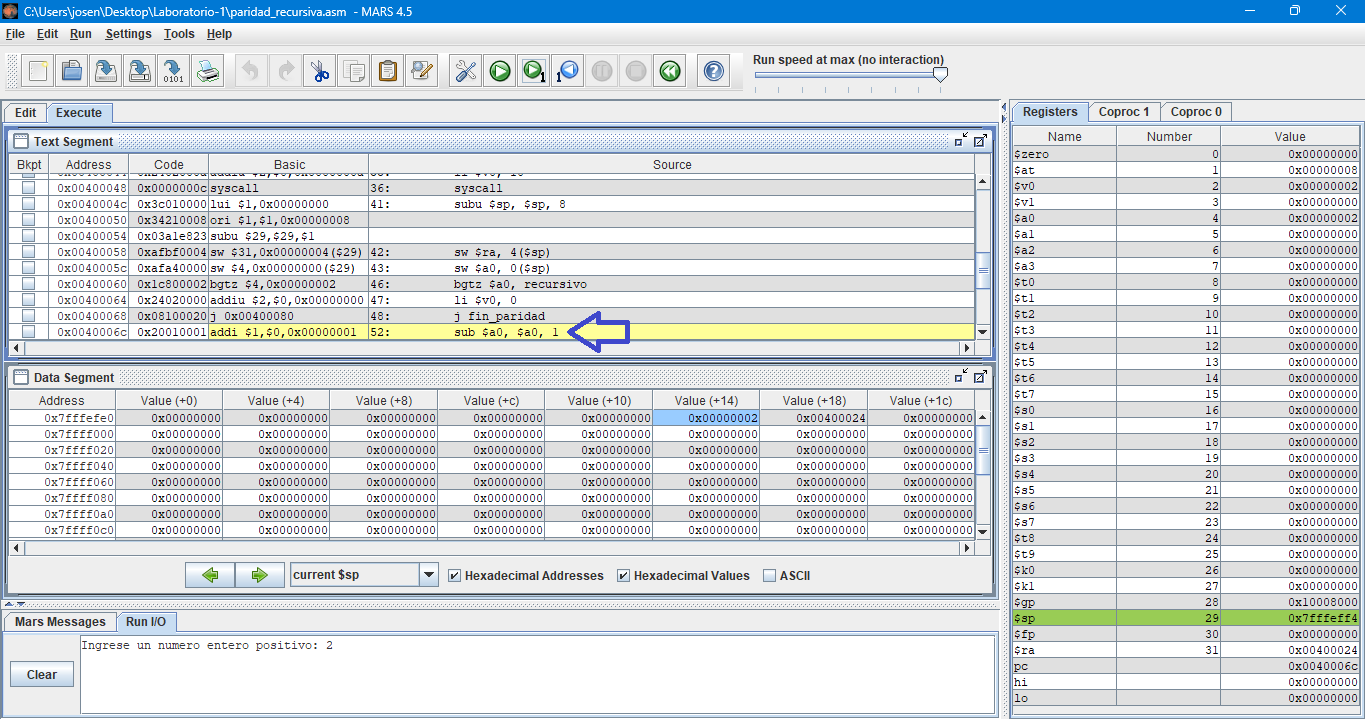
\includegraphics[width=1.0\textwidth]{./media/image6.png}

-Paso 6: El programa al llegar a la etiqueta ``\emph{recursivo}'' llega
a la linea 52: le resta 1 a \$a0 (por lo tanto \$a0 ahora es 1) y salta
a la etiqueta ``\emph{paridad}''.

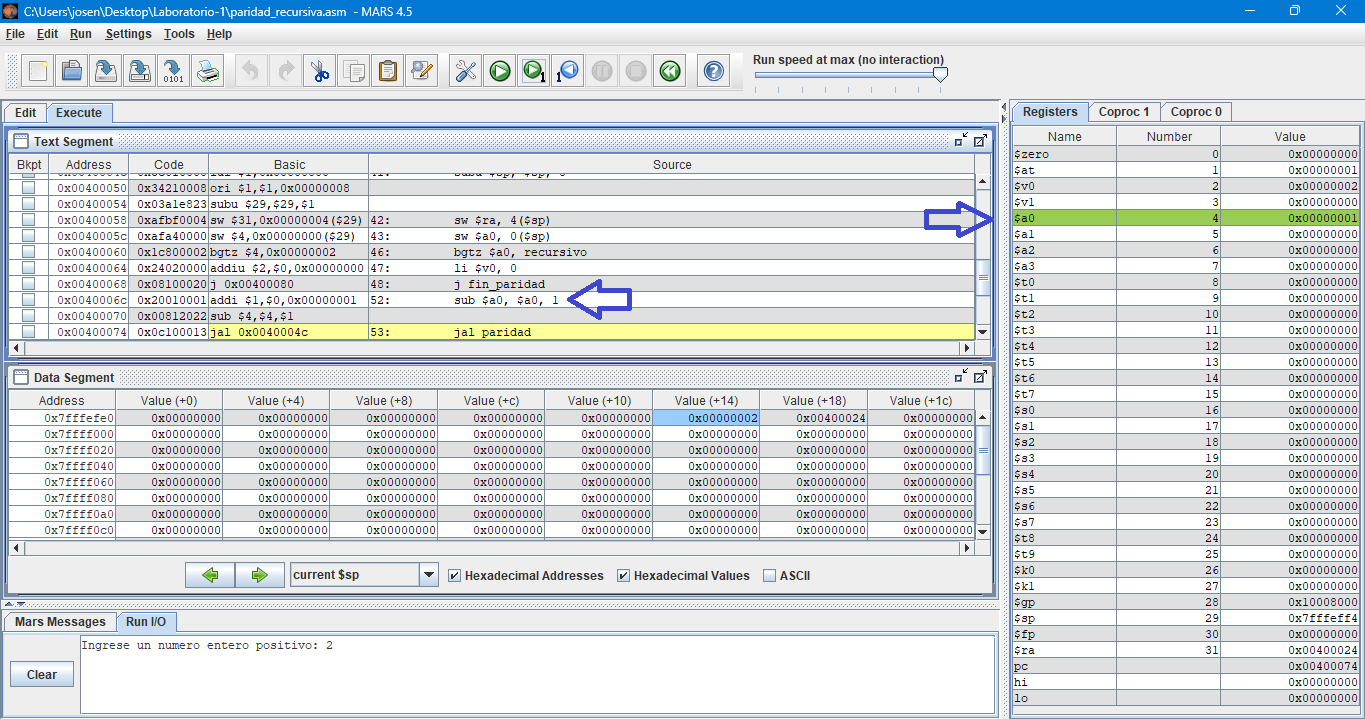
\includegraphics[width=1.0\textwidth]{./media/image7.png}

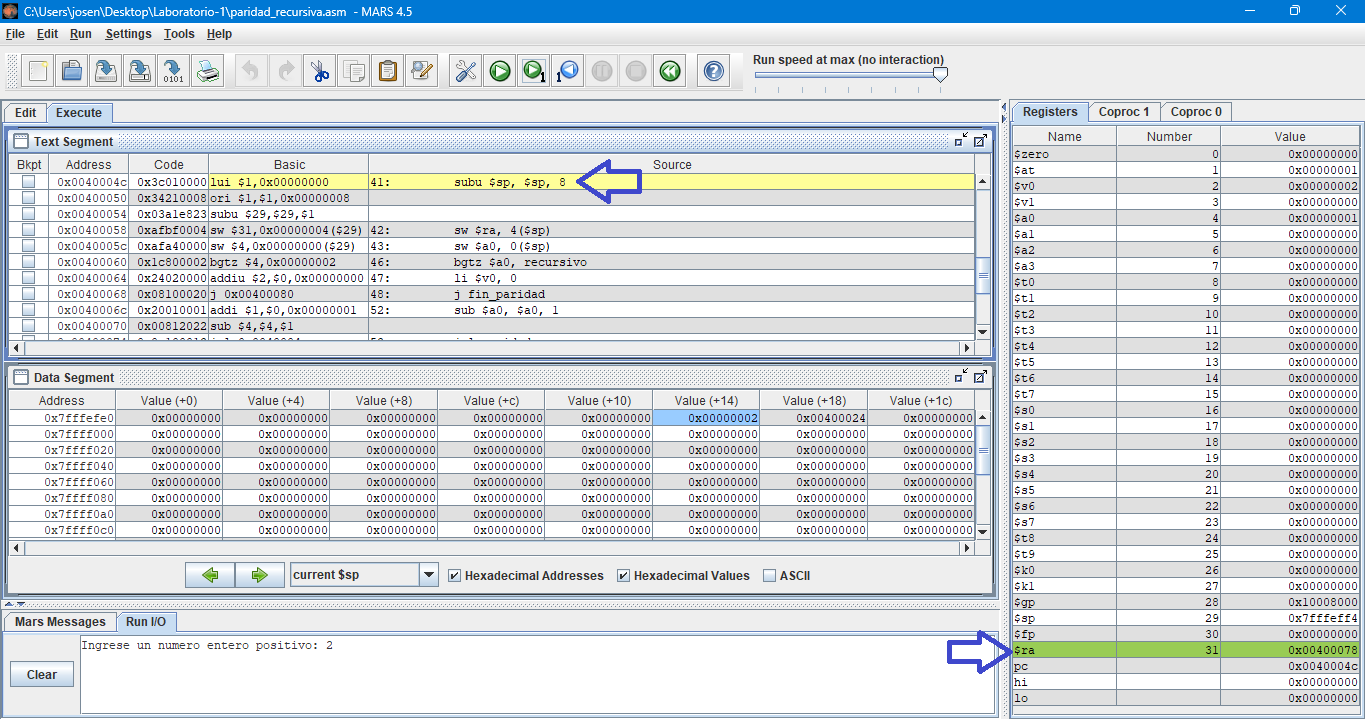
\includegraphics[width=1.0\textwidth]{./media/image8.png}

-Paso 7: Los pasos (4), (5) y (6) se repiten hasta que \$a0 sea igual a
cero. Por cada paso el valor del puntero \$sp va cambiando, lo que
significa que se esta usando otra ``caja'' de memoria.

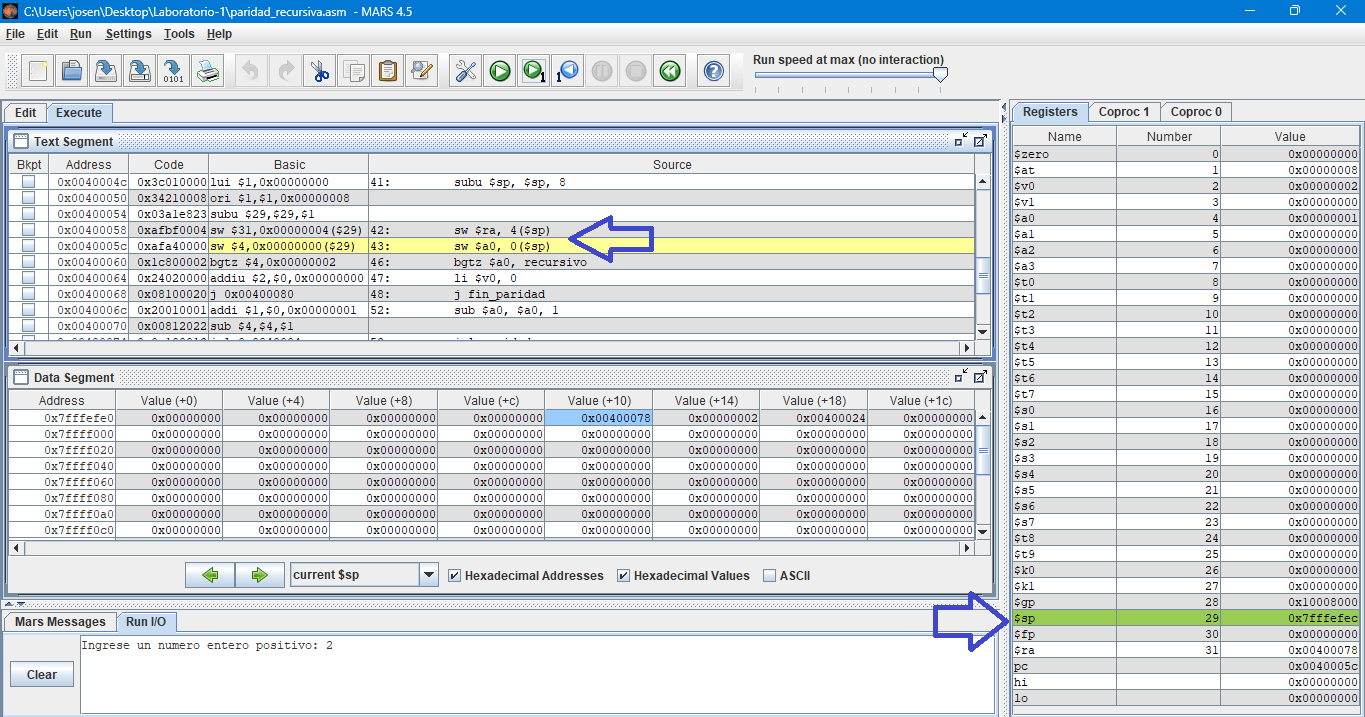
\includegraphics[width=1.0\textwidth]{./media/image9.png}

-paso 8: Tras varias pasadas, el valor del registro \$a0 ahora es cero y
por lo tanto la linea 46: (la de operación bgtz) da falso y no salta
hacia la etiqueta ``\emph{paridad}'', en cambio sigue por las lineas 47:
y 48:.

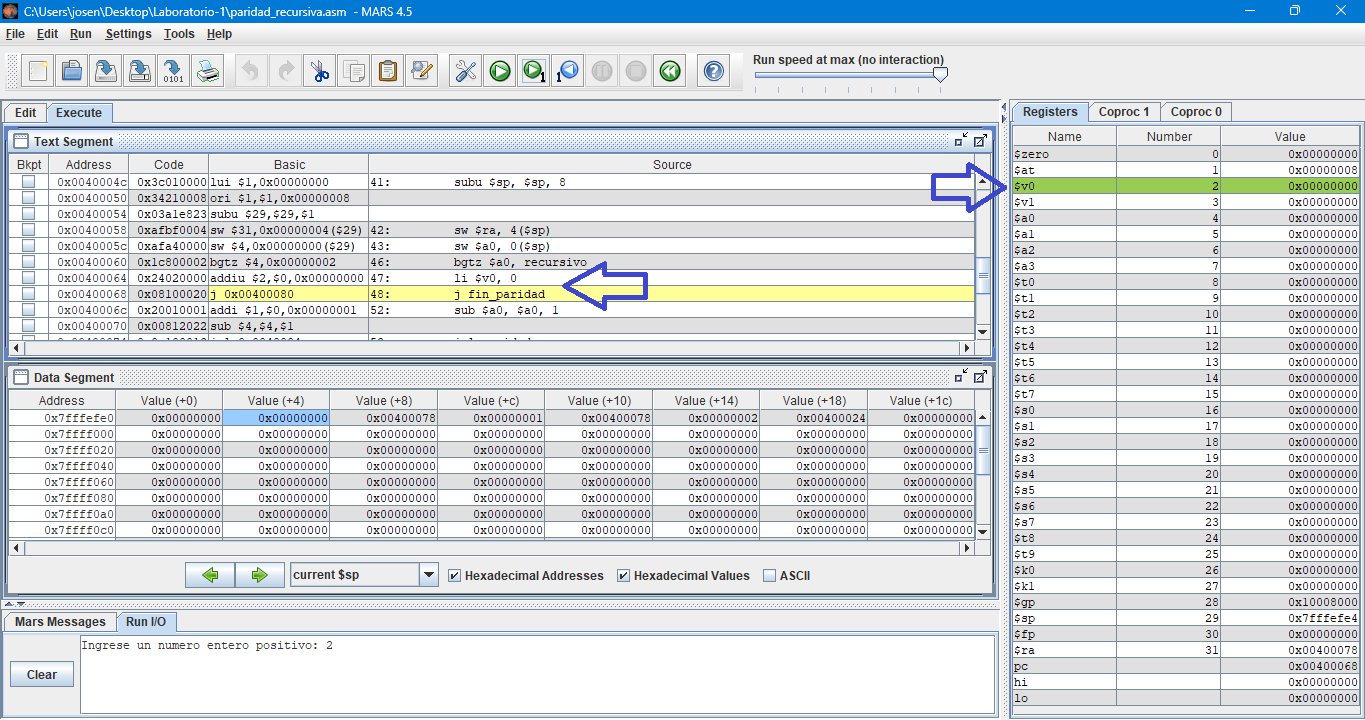
\includegraphics[width=1.0\textwidth]{./media/image10.png}

-Paso 9: El programa al llegar a la linea 48: salta hacia la etiqueta
``\emph{fin\_paridad}'' en donde se recupera el valor de puntero \$sp
para ir regresando a la ``caja'' anterior, así hasta regresar a la
``caja'' original (el main).

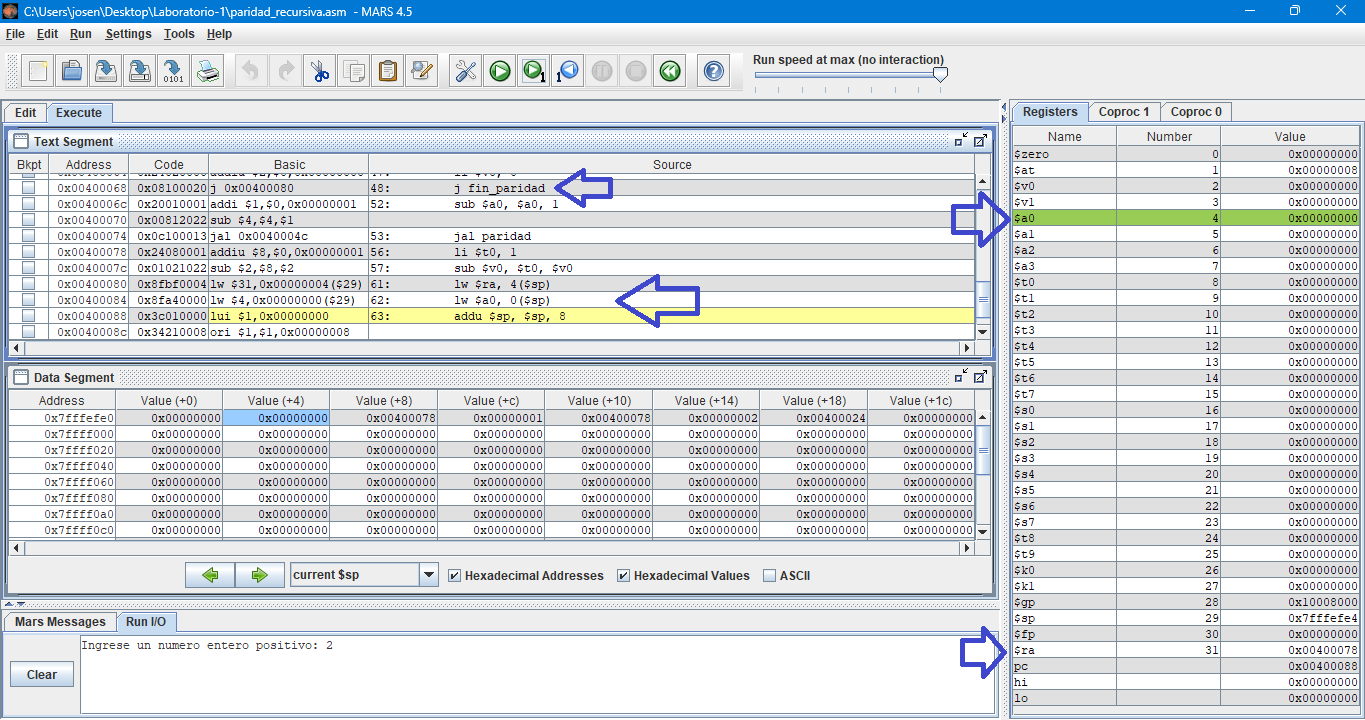
\includegraphics[width=1.0\textwidth]{./media/image11.png}

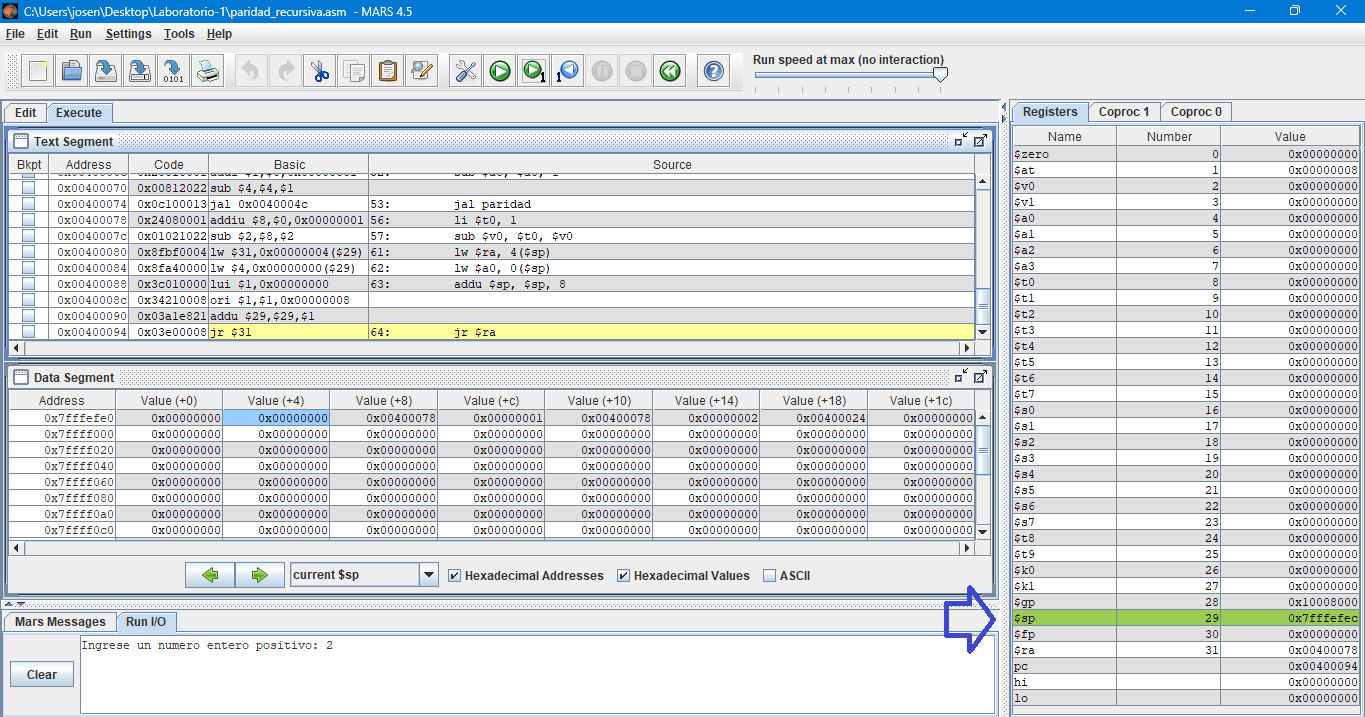
\includegraphics[width=1.0\textwidth]{./media/image12.png}

-Paso 10: El programa cuando regresa al main pasa por las lineas 25: a
28:, le asigna al registro \$v0 el valor 4 para asi escribir el mensaje
``\emph{La paridad es:}''. Luego le asigna al registro \$v0 el valor 1
(usado para escribir un entero) y escribe el valor resultante.

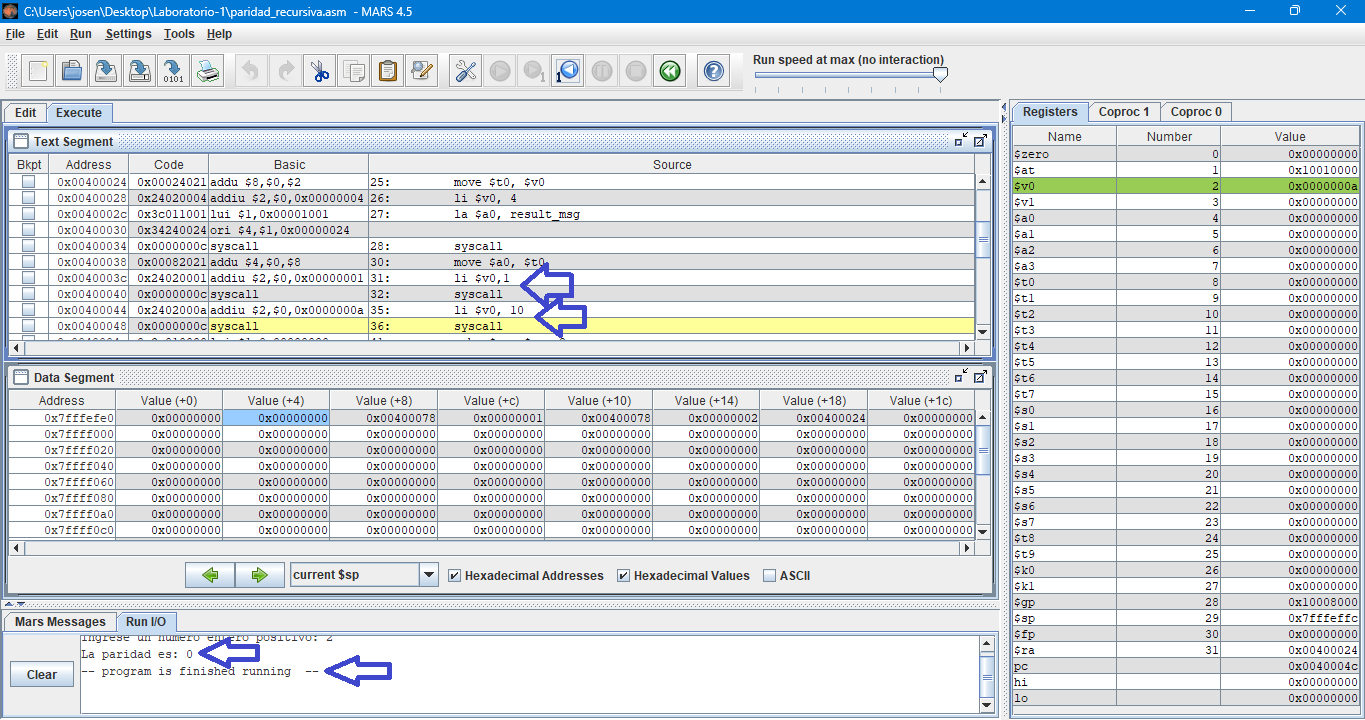
\includegraphics[width=1.0\textwidth]{./media/image13.png}

Iterativo:

-Paso 1: Tras ensamblado el programa, este llega a la linea 10: y le
asigna a \$v0 el valor 4 (usado para escribir un string) para asi
escribir el texto ``Ingrese un numero entero positivo''.

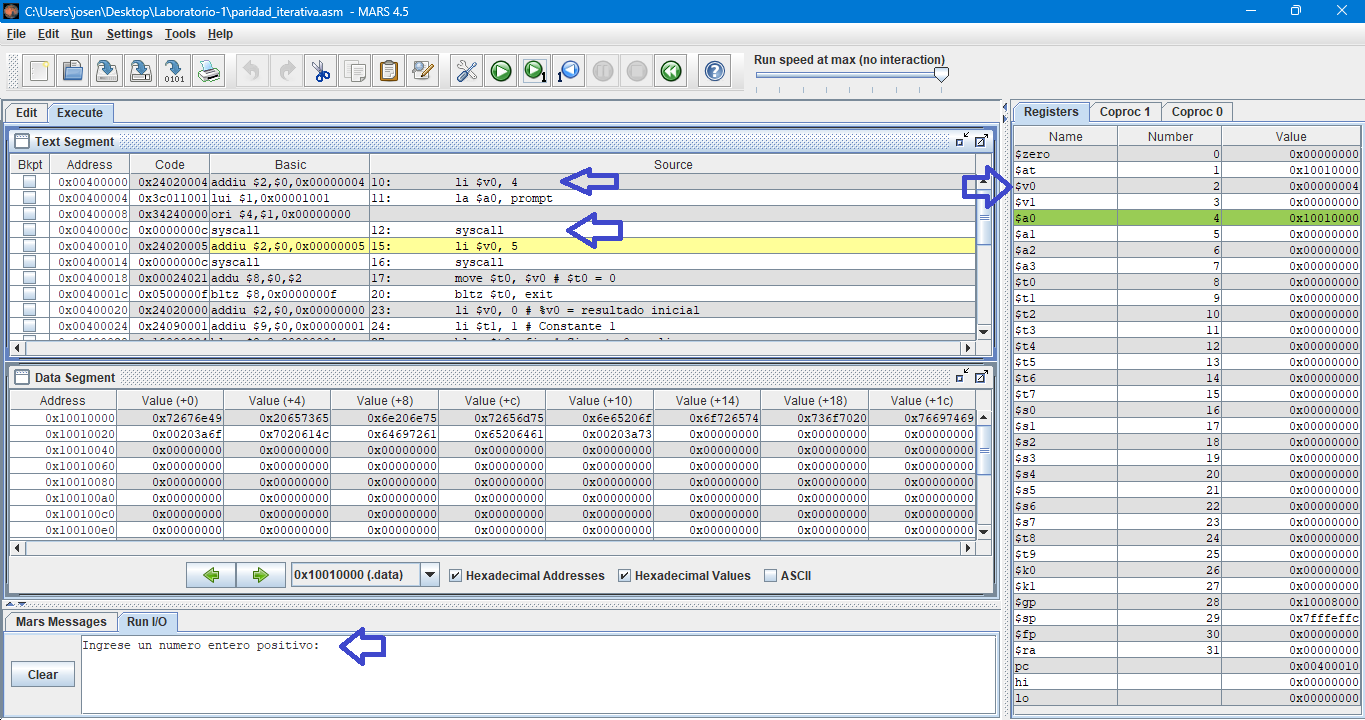
\includegraphics[width=1.0\textwidth]{./media/image14.png}

-Paso 2: Luego llega a la linea 15: y le asigna a \$v0 el valor 5 (usado
para recibir un entero) para asi esperar que el usuario ingrese un
numero.

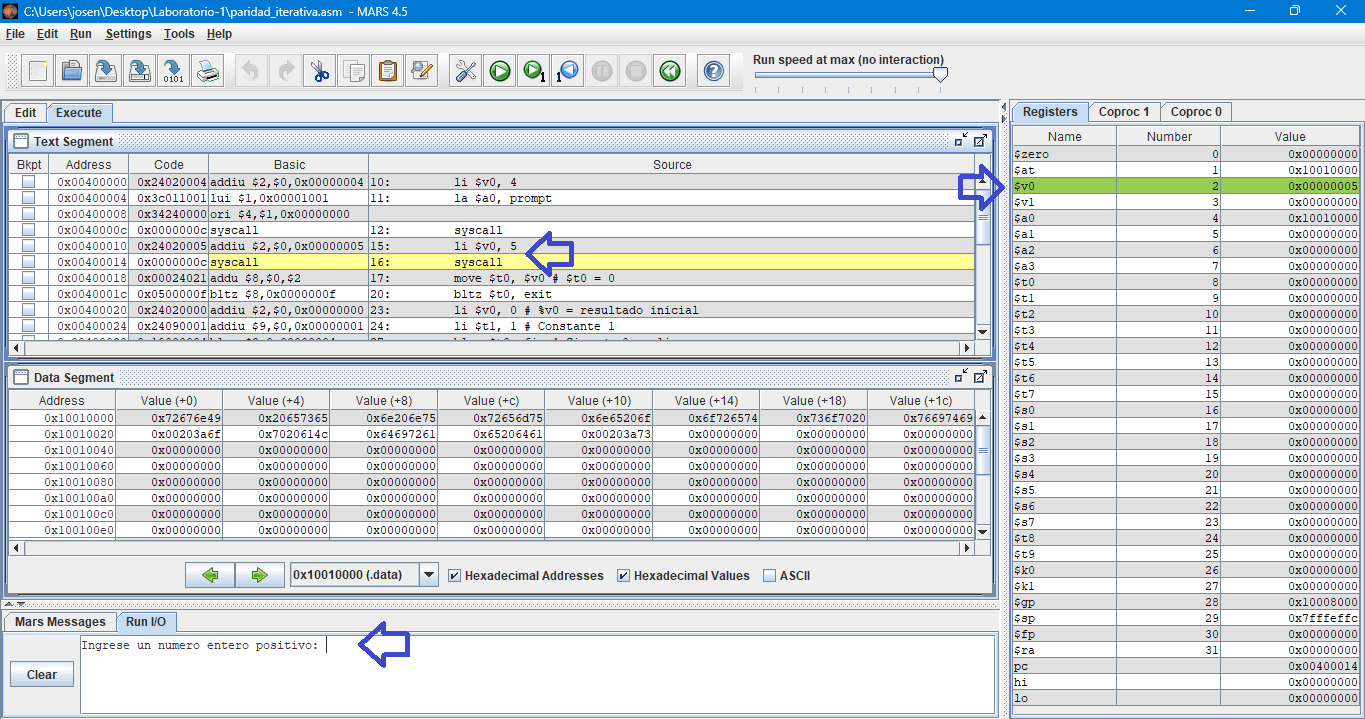
\includegraphics[width=1.0\textwidth]{./media/image15.png}

-Paso 3: Tras recibir el valor, el programa llega a la linea 27: donde
usa la funcion blez para saber si el valor n ingresado ya llego a cero.
Si todavia no llego a cero sigue a las lineas 28: y 29: en donde se le
resta uno al valor n (n-1).

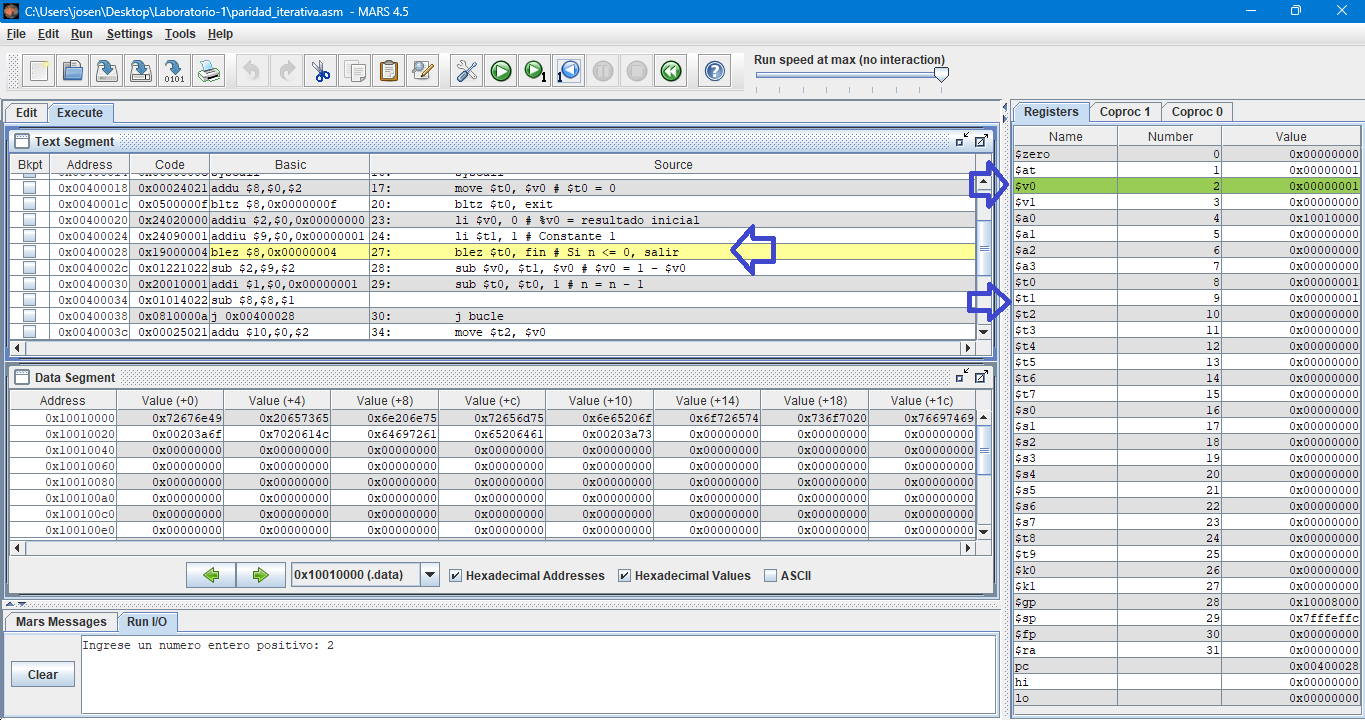
\includegraphics[width=1.0\textwidth]{./media/image16.png}

-Paso 4: El programa llega a la linea 30: en donde se aplica el salto
hacia la etiqueta ``bucle'' (j bucle). Los pasos (3) y (4) se repiten
hasta que el valor n se vuelva cero.

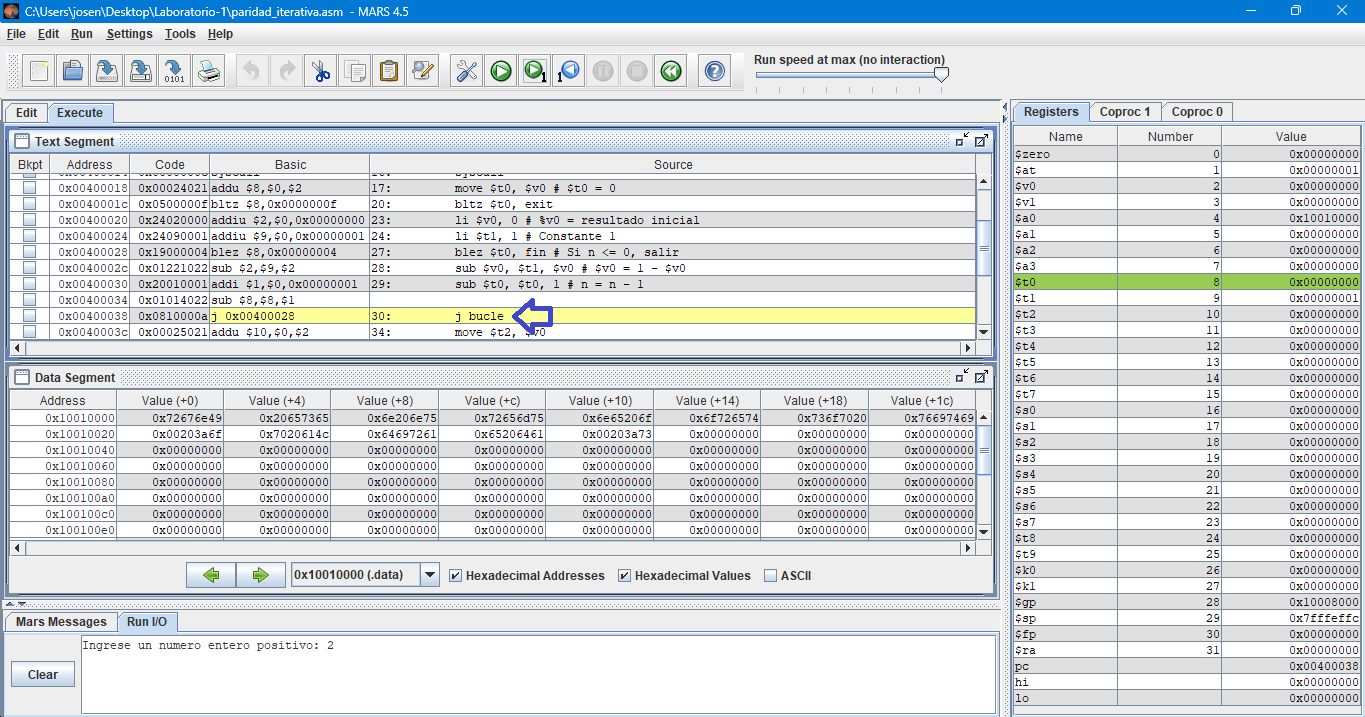
\includegraphics[width=1.0\textwidth]{./media/image17.png}

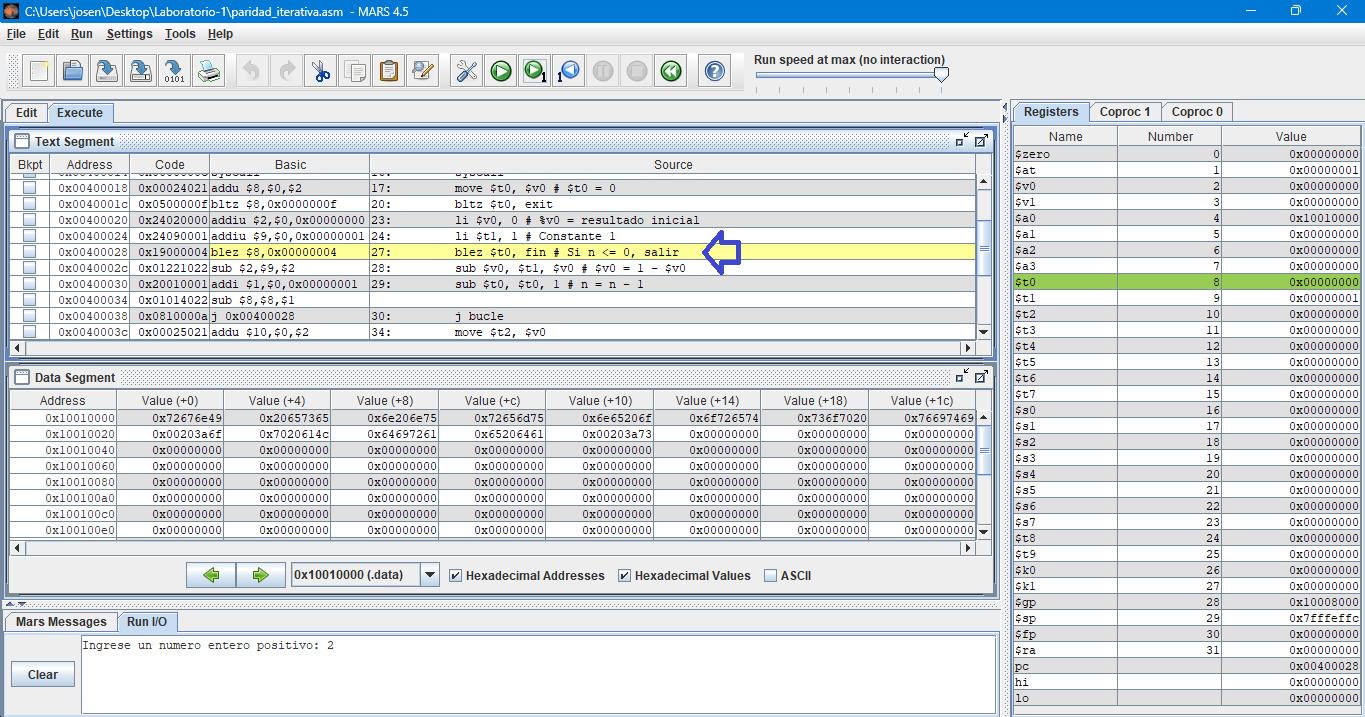
\includegraphics[width=1.0\textwidth]{./media/image18.png}

-Paso 5: Tras que se repita el paso (4) hasta que n se vuelva cero, la
linea 27: de funcion blez es verdad y entonces salta hacia la etiqueta
``salir''.

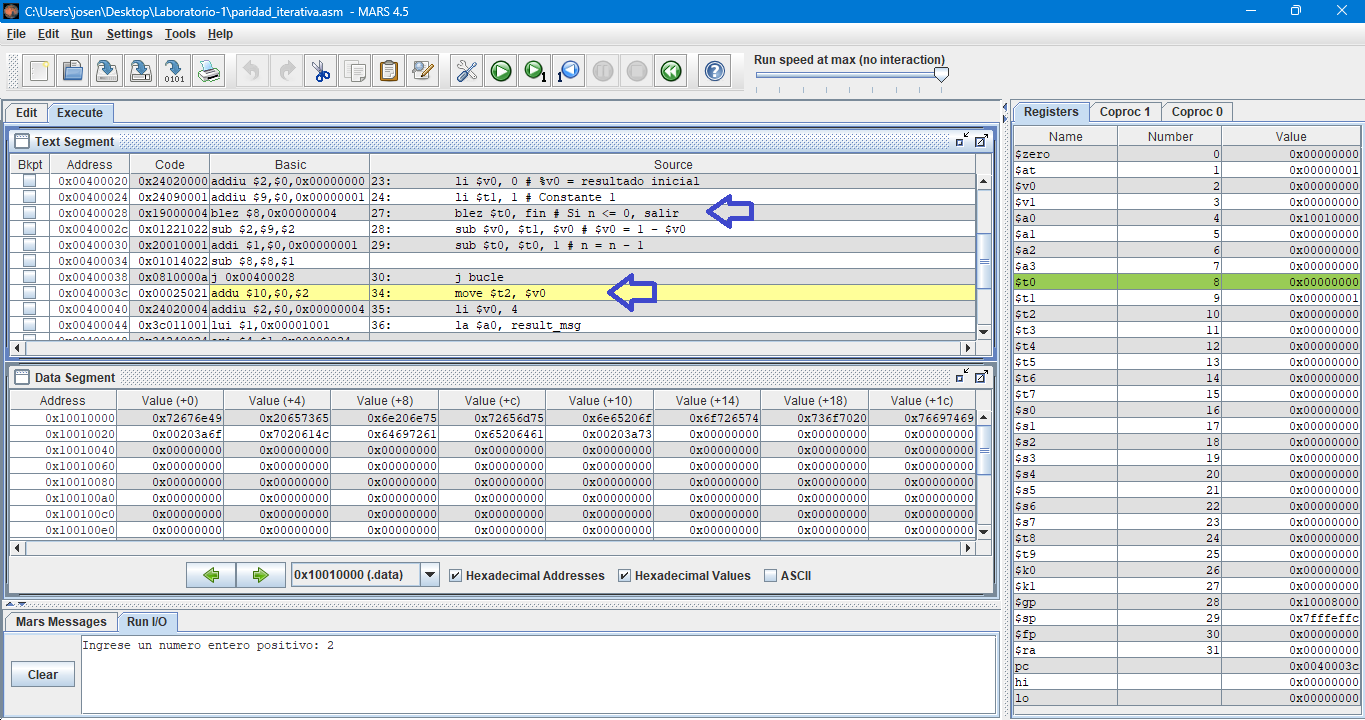
\includegraphics[width=1.0\textwidth]{./media/image19.png}

-Paso 6: Tras saltar a la etiqueta ``salir'' llega a las lineas 34: a
37: en donde se prepara el mensaje ``La paridad es: ''. Luego finalmente
llega a las lineas 39: a 45: en donde retorna el valor resultante.

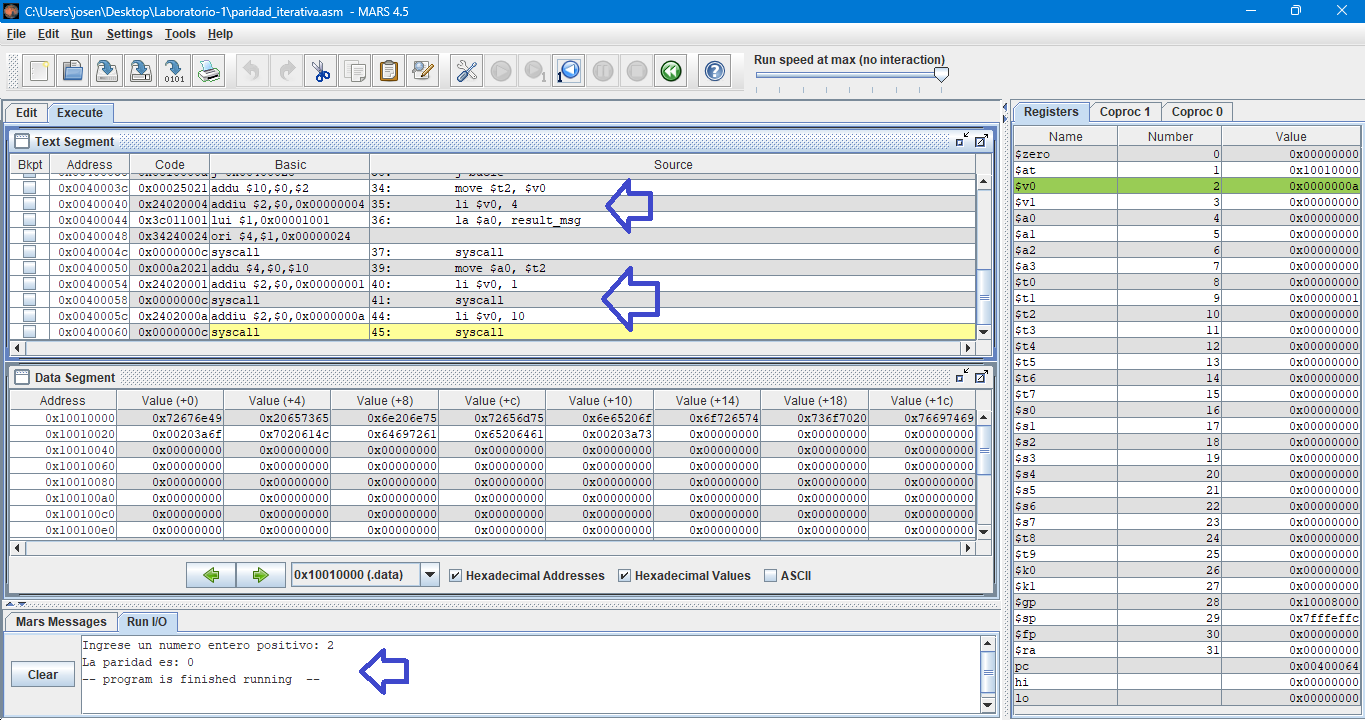
\includegraphics[width=1.0\textwidth]{./media/image20.png}

6. Justificar la elección del enfoque (iterativo vs. recursivo) según
eficiencia y claridad

- \textbf{Eficiencia} (\textbf{Ganador: Iterativo}): Es
indiscutiblemente más eficiente. No requiere el \emph{overhead} de
gestión (push/pop) ni el riesgo de desbordamiento. Para sistemas
embebidos, donde la memoria es un recurso crítico, el enfoque iterativo
es obligatorio.

- \textbf{Claridad} (\textbf{Ganador: Recursivo}): La recursividad
brilla en la legibilidad. Si miras la definición matemática del
problema:

\textbf{paridad(n) = 1 -- paridad(n -- 1)}

El código recursivo es una traduccion casi literal de la fórmula. Es
mucho más facil de auditar y mantener para problemas matemáticos
complejos o estructuras de datos (como árboles).

\textbf{Conclusión técnica}: Elegir uno obre otro es un
\emph{trade-off}. En entornos de producción con restricciones de
memoria, la iteración es el estándar. En entornos de prototipado donde
la elegancia y la rapidez de desarrollo son prioridad, la recursión es
una herramienta poderosa.

7. Análisis y discusión de los resultados

- \textbf{Sobre el entorno MARS}: El simulador nos permite ver el
proceso que toma el procesador al ejecutor los programas (lo que nos
ayudo a entender mejor el \textbf{MIPS32}).

- \textbf{Resultados observados}: Al probar con valores pequeños, ambos
enfoques entregaron los mismos resultados correctos. Sin embargo, al
monitorear el registro \textbf{\$sp} en la versión recursiva, fue
evidente el crecimiento de la pila, confirmando que la recursión es una
herramienta poderosa pero costosa en términos de memoria.

- \textbf{Aprendizaje principal}: Como dicho antes, el usar el entorno
MARS para desarrollar y ejecutar los programas y el ver como se
comportan los registros y pilas a nivel del procesador nos permitio
entender un poco mejor el como funciona el lenguaje de alto nivel, su
idea y el como se puede usar de mejor manera.

Conclusión

Tras finalizar el desarrollo y la experimentación en MARS, se concluye
que la elección entre una solución iterativa y una recursiva no es
meramente una cuestión de estilo, sino una decisión de ingeniería
condicionada por las restricciones del sistema.

Si bien la recursividad ofrece una expresividad matemática superior y
una implementación más cercana a la definición lógica del problema, su
costo en memoria y el riesgo inherente de \emph{stack overflow} la
posicionan como una herramienta de uso cuidadoso. En contraparte, la
implementación iterativa demuestra ser la opción robusta y eficiente al
mantener un uso constante de la memoria (\emph{\textbf{O(1)}}), lo que
garantiza la estabilidad en la ejecución, independientemente de la
magnitud de la entrada.

En última instancia, este laboratorio subraya la importancia de la
convención de llamadas (\emph{calling convention}) y el papel vital que
desempeñan los registros y la pila en la ejecución de cualquier
programa. El dominio de estos conceptos es, sin duda, la diferencia
entre un código funcional y uno optimizado, capaz de operar de manera
eficiente en la arquitectura subyacente.

\end{document}
